\chapter{Introdução} \label{Introducao}

\section{Endereços e Geocodificação}
 
\epigraph{Quase tudo o que acontece, acontece em algum lugar. Saber o local onde algo acontece pode ser fundamental.}{\cite{longley2013}}

Em \cite{longley2013}, os autores exploram a relação entre a humanidade e a localização. Para eles, é evidente que a maior parte das atividades humanas ocorre no planeta Terra, e, portanto, a vida está profundamente ligada à localização. Assim sendo, compreender e manipular informações geográficas é essencial para qualquer aplicação que envolva a humanidade. Além disso, os autores explicam que decisões importantes podem ter consequências geográficas. Um exemplo disso seria uma transação financeira que, em casos extremos, poderia desencadear uma crise econômica em uma região específica.

O endereço é a principal maneira de conceitualizar a localização no mundo atual\cite{Zamberg2009}. Isso ocorre devido ao fato de os endereços serem utilizados em diversas aplicações de diferentes áreas de estudo, como na saúde \cite{AmericaJournal2001, Kypri2009, Mazumdar2008}, nas ciências sociais \cite{Chow2011}, na análise criminal ou judiciária \cite{Olligschlaeger1998}, na análise ambiental \cite{Gilboa2006}, na ciência da computação \cite{Zamberg2009}, na economia \cite{Whitsel2006} e em outros campos.

Para atingir esse objetivo, é necessário criar uma representação computacional do endereço para que as aplicações possam utilizá-la. A representação mais comum é a utilização de coordenadas x e y em um plano, geralmente representando latitude e longitude. Esse processo de transformação de um endereço nessas coordenadas é chamado de Geocodificação ou Georreferenciamento e envolve três etapas \cite{Zamberg2009}:

\begin{itemize}
   \item Processamento do endereço de entrada: o endereço é lido, dividido em componentes (rua, número, bairro, etc.), padronizado e cada campo é atribuído a uma categoria; por fim, as categorias necessárias são indexadas.
   \item Busca na base de referência: com base no algoritmo escolhido, é realizada uma busca na base de referência para selecionar e classificar potenciais candidatos como resposta.
   \item Seleção do(s) candidato(s) para resposta: após a busca, a classificação gerada é analisada e os melhores candidatos são selecionados.
\end{itemize}

Além de representar um endereço computacionalmente, o georreferenciamento utilizando latitude e longitude oferece várias vantagens \cite{longley2013}:

\begin{itemize}
   \item Precisão espacial: é capaz de indicar com alta precisão a localização de um determinado endereço.
   \item Cálculos de distância: como é um sistema espacial, permite a obtenção de distâncias e, por consequência, o cálculo de outras métricas para o endereço.
   \item Compreensão global: é um sistema usado mundialmente e, geralmente, é mais fácil de identificar e entender.
\end{itemize}

Apesar de todas as vantagens e aplicações, o processo de geocodificação pode levar a informações incorretas. Essas informações conflitantes são chamadas de ``incertezas'' \cite{longley2013}. Para compreender o que é a incerteza, é necessário considerar outros aspectos das falhas de informação. Nesse contexto, são introduzidos os seguintes conceitos:

\begin{itemize}
   \item Erro: a diferença entre a referência e o obtido.
   \item Falta de acurácia: a diferença entre a realidade e nossa representação dela.
   \item Ambiguidade: quando um único valor está presente em mais de um objeto.
   \item Indefinição: a falta de informações necessárias.
\end{itemize}

Dados estes termos, podemos definir a incerteza como: ``a medida da compreensão do usuário sobre a diferença entre o conteúdo de um conjunto de dados e os fenômenos reais que os dados devem representar'' \cite{longley2013}. Em outras palavras, a incerteza é uma medida que descreve o nível de compreensão do usuário em relação ao conjunto de dados obtidos e à realidade que esses dados têm a intenção de representar. A figura \ref{fig:incerteza} apresenta uma visão conceitual da incerteza, onde cada processo muda um pouco a realidade, sendo assim a representação final tem sempre um nível de incerteza que está relacionado com o filtro aplicado em cada etapa. Por exemplo, a incerteza entre o mundo real e a concepção da realidade está relacionada ao filtro I1 que distorce a realidade para que seja possível a concepção.  A partir desses conceitos, a incerteza foi aceita como uma métrica apropriada para avaliar a qualidade dos Sistemas de Informação Geográfica (SIG) \cite{longley2013}.

\begin{figure}[ht]
   \centering
   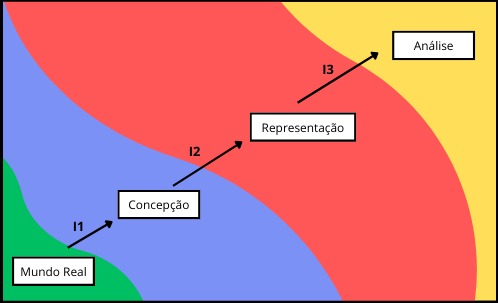
\includegraphics[width=0.8\textwidth]{Figuras/incertezaMeu.jpeg}
   \caption{Adaptada do livro \cite{longley2013}. Visão conceitual da incerteza}
   \label{fig:incerteza}
\end{figure}

Apesar da incerteza ser uma métrica de importância significativa, sua mensuração é complexa. A incerteza envolve medidas que são subjetivas e podem variar de acordo com cada indivíduo avaliado. 

%Por essa razão, optamos por utilizar a medida de erro para representar a qualidade da geocodificação. Embora essa medida não seja equivalente à incerteza, ela é uma parte integrante da mesma. Dentro das componentes que compõem a incerteza, a medida de erro é a mais objetiva e fácil de mensurar.

Diversas empresas e organizações de renome, como New York Times, CNN, BMW, Toyota, Strava, Microsoft, Uber, Fiat, Jeep, e TerraLAB,  utilizam informações geográficas para o desenvolvimento de suas aplicações \cite{ors, terralab, mapbox, tomtom}. Essas aplicações utilizam endereços geocodificados para criar mapas, rotas, áreas de abrangência, relatar locais, divulgar eventos, entre outras funcionalidades. Isso ressalta a grande importância da geocodificação e como a qualidade desse processo impacta significativamente o que é produzido nesses locais. Para adquirir informações relacionadas a endereços, elas utilizam da geocodificação obtida por meio de APIs online.

\section{APIs de Geocodificação e Análise de qualidade}

Por muitos anos, a principal maneira de obter informações geográficas era através de software SIG. Um Sistema de Informação Geográfica (SIG) é um conjunto de ferramentas capazes de analisar e integrar dados geográficos, permitindo acesso fácil a dados para os usuários, sem depender de ferramentas como o GPS \cite{stein2021geoprocessamento}.

Embora os SIG tenham sido a ferramenta convencional por muitos anos, utilizar esse método para geocodificação requer um profissional capacitado. A ferramenta demanda o pré-processamento dos dados, criação de um localizador de endereços, customização de parâmetros, controle de qualidade e correção manual de falhas. Todo esse processo é custoso para o usuário comum. Por essa razão, a geocodificação utilizando ferramentas online retira do usuário grande parte da responsabilidade, como a manutenção da base, tornando assim o processo de obtenção de informações menos oneroso \cite{Chow2016}.

Apesar de a geocodificação online ser mais simples de utilizar, para que o SIG seja substituído por ela, deve-se considerar sua qualidade em relação à qualidade do SIG. Em \cite{Chow2016}, são avaliadas oito ferramentas de geocodificação, sendo duas delas SIGs e as demais ferramentas da internet. As ferramentas utilizadas foram: SRI ArcGIS Address Locator, CoreLogic PxPoint, Google Maps API, Yahoo! PlaceFinder, Microsoft Bing, Geocoder.us, Texas A and M University Geocoder e OpenStreetMap (OSM). Para calcular o erro, uma base de referência foi utilizada, contendo informações descritivas do endereço (rua, número, cidade etc.) e informações geográficas (latitude e longitude). Essa base é considerada a referência, pois os dados de latitude e longitude foram obtidos manualmente (por GPS ou pesquisa manual). Chamaremos essa e outras bases de referência de "base padrão ouro". A base em questão contém 940 endereços do estado do Texas, Estados Unidos da América (EUA), sendo que 78 destes são da região Central Texas, região considerada importante para o autor. O erro de cada endereço geocodificado foi calculado como a distância euclidiana de dois pontos, sendo eles, o ponto referência e o ponto obtido a partir da geocodificação.

O estudo evidenciou que não há diferença significativa entre as ferramentas online e os SIGs. Tanto os SIGs quanto as ferramentas online apresentaram média e desvio padrão de erro semelhantes. Além disso, a taxa de resposta (ou seja, quantos endereços receberam uma resposta da ferramenta utilizada) variou entre 97,8\% e 100\%, o que é considerado satisfatório. Dessa forma, o estudo obteve êxito ao mostrar evidência que as ferramentas online podem ser utilizadas como substitutas dos SIGs.

Apesar de \cite{Chow2016} ter apresentado resultados significativos, o estudo apresenta algumas limitações. A principal delas é a quantidade de dados utilizada para a avaliação, além do foco restrito a uma única região (Texas, EUA). 

Outro estudo importante é \cite{Clodoveu2011}, que faz uma avaliação da qualidade da geocodificação da Google Maps API fornecida pela Google Cloud Platform \cite{GCP}. Nesse estudo, os autores utilizam uma base padrão ouro com os dados de Belo Horizonte, cidade de Minas Gerais, estado do Brasil para essa avaliação. A base conta com mais de 540 mil endereços da cidade e é mantida pela empresa de informática e informação do município de Belo Horizonte - Prodabel \cite{Prodabel}. A empresa atualiza os dados mensalmente e tem parceria com outras 26 empresas para manter a base o mais correta possível. Ela conta com informações descritivas, sociais e espaciais do endereço. Para medir o erro, foi calculada a distância euclidiana dos pontos geocodificados para os pontos originais. A partir do erro, o estudo faz análises espacias do erro e também relaciona a acurácia descrita pela API com o erro gerado. O estudo mostrou que o Google Maps API tem taxa de acerto de 74,7\%, considerando que acertou se o erro for menor de 150 metros. Outra descoberta foi que o erro é menor nas áreas centrais da cidade, e maior na periferias. Os autores também tentaram fazer uma relação entre erro e renda, porém não foi possível vizualizar nenhuma relação direta.

Apesar das descobertas importantes, o estudo apresenta limitações notáveis. Primeiramente, ele se restringe à análise de apenas uma API de geocodificação. Além disso, o estudo se concentra exclusivamente em uma cidade brasileira, o que restringe a generalização dos resultados. 

\section{APIs de Geocodificação e  formatação das entradas}

A maioria das APIs possuem recomendações de formato de entrada que podem ser encontradas na documentação das mesmas. 

Apesar das recomendações nas documentações das APIs, existem observações relacionadas à possibilidade de utilizar formatos de entrada diferentes dos apresentados, bem como a falta de informações abrangentes. Os geocodificadores das APIs são preparados para lidar com essas modificações, no entanto, a qualidade pode ser comprometida.

Com isso em mente, em trabalhos anteriores a equipe de análise de dados do TerraLAB \cite{terralab} conduziu uma série de experimentos para avaliar os impactos da modificação na ordem dos endereços de entrada nas APIs \cite{relatorioDeA}. Foram realizados 10 experimentos, nos quais o formato de entrada variou. Para avaliar a qualidade dos dados produzidos, foi utilizada a métrica de ``dentro e fora da cidade''. Se o endereço resultante estivesse dentro dos limites da cidade em questão, considerava-se que a API acertou naquele endereço; caso contrário, considerava-se um erro. No total, foram utilizados 100 endereços. Além disso, foram utilizadas as seguintes APIs: Mapbox, TomTom, Here e ORS. O trabalho concluiu que a maioria das APIs não apresenta uma diferença significativa ao mudar a formatação de entrada, exceto a API Mapbox, que apresentou uma melhora significativa para a formatação estado, cidade, rua e número.

Embora o trabalho apresente questionamentos importantes, ele possui uma série de limitações. A principal delas é a quantidade de endereços avaliados, que é insuficiente para gerar conclusões concretas. Além disso, apenas uma métrica foi avaliada. Dessa forma, não é possível determinar se a qualidade é realmente impactada pela formatação dos dados de entrada ou se isso impacta apenas essa métrica específica.
 
Encontrar a melhor forma de organizar a entrada para os geocodificadores é uma meta de diversos estudos. Em \cite{KUCUKMATCI2018}, é proposto um método de padronização da entrada que melhora o resultado da geocodificação. Para validar o método, eles utilizaram 233 endereços de escolas em Eskishehir, uma cidade da Turquia, para a qual as coordenadas corretas são conhecidas. Foi criado um dicionário contendo as principais abreviações e falhas de escrita, que foram utilizadas em métodos de processamento de linguagem natural (PLN). Os métodos de PLN foram empregados para gerar o endereço padronizado a partir do endereço inicial, de acordo com o dicionário. Além disso, foram utilizados dois geocodificadores, o ArcGIS e o Google Maps. A qualidade da geocodificação foi avaliada com base na distância euclidiana entre o ponto geocodificado e o ponto de referência, considerando acerto quando o erro foi menor que 100 metros.

O estudo demonstrou que o método de padronização reduziu significativamente o erro da geocodificação e aumentou as taxas de acerto, com uma diferença variando de 6\% a 20\%, dependendo do formato e da API utilizados.

Apesar dos resultados significativos, o estudo apresenta algumas limitações. As principais são a quantidade de dados avaliados e o foco em uma cidade específica, não sendo possível, dessa forma, generalizar os resultados para além desse contexto.

A padronização do formato de endereços é um tópico de interesse para organizações em todo o mundo. Algumas organizações têm se esforçado para estabelecer um padrão no formato de endereços. A Organization for the Advancement of Structured Information Standards (OASIS) é mencionada como uma organização bem-sucedida no desenvolvimento de especificações que incluem a padronização de endereços. Essa padronização é utilizada no geocodificador do Google Maps \cite{GoogleDoc}. No entanto, vale ressaltar que nem todas as organizações adotam o mesmo padrão e muitas delas mantêm suas próprias convenções de formatação \cite{behr2010}.

Todas essas considerações evidenciam que, apesar dos esforços em busca de um padrão na formatação de endereços com o objetivo de melhorar sua qualidade, ainda há muito a ser feito. Além disso, a padronização é influenciada por diversos fatores, incluindo o geocodificador utilizado e a região geocodificada. 

\section{Objetivos}

A avaliação de qualidade é uma frente crucial do presente trabalho. Em relação a ela, os principais problemas levantados foram a quantidade de dados utilizados, a quantidade de APIs avaliadas e as regiões abarcadas pela análise. O presente trabalho busca abordar essas limitações ao conduzir a análise em uma região diferente do mundo, com ênfase no Brasil, e ampliando a quantidade de dados avaliados. Avaliaremos quatro APIs de geocodificação de grande impacto no mercado, utilizando duas bases de dados extensas. Além disso, nosso estudo incluirá a cidade de Belo Horizonte e a região metropolitana de São Paulo, proporcionando uma maior diversidade regional à análise. Dessa forma, pretendemos oferecer uma avaliação mais abrangente e representativa das ferramentas de geocodificação online (GeoAPIs).

Além disso, buscamos ir além por meio de duas abordagens distintas.

A primeira consiste em investigar se existe alguma métrica que poderia substituir o erro. Em outras palavras, buscamos identificar se há alguma medida que esteja correlacionada com o erro, de modo que possamos utilizá-la como alternativa à mensuração do erro em si.

Conscientes de que a obtenção do erro requer um valor de referência, considerado suficientemente preciso para calcular o erro, reconhecemos que a aquisição de informações geográficas de alta qualidade é uma tarefa desafiadora. A forma mais confiável de reduzir a incerteza é a coleta de dados in loco, com a utilização de dispositivos GPS.
Por outro lado, medidas de discrepância dependem apenas dos valores que estão sendo avaliados. Para entender melhor essa afirmação, precisamos entender o que é discrepância no conceito geral e como ela é aplicada na nossa pesquisa. Discrepância é o mesmo que discordância ou desigualdade \cite{klein2015}. Sendo assim, a discrepância reflete o desacordo entre duas ou mais coisas. No contexto da pesquisa, tratamos como discrepância as diferenças de informações entre as APIs. Então, as medidas de discrepância são aquelas que medem de alguma forma essa diferença. Dessa forma, temos medidas que necessitam apenas das informações geradas pelas APIs, facitando a obtenção das métricas em relação ao erro.

Com acesso às medidas de discrepância e o erro, um dos nosso objetivos é verificar se existe alguma relação entre eles. Correlação é definida como: "grau de relação entre as variáveis, que procura determinar quão bem uma equação linear, ou de outra espécie, descreve ou explica a relação entre as variáveis"\cite{spiegel2009}.

A segunda abordagem visa compreender as causas do erro e identificar a melhor forma de configurar as entradas nas APIs a fim de minimizá-lo. Como abordado anteriormente, a melhor forma de entrada para as APIs ainda é um estudo em aberto. A qualidade dos dados depende do geocodificador utilizado e da região avaliada. Nesse contexto, o presente trabalho tem como propósito propor e avaliar formatos de padronização que sejam aplicáveis à região do Brasil e aos geocodificadores utilizados no Laboratório TerraLAB.

Dado o contexto, o principal objetivo deste trabalho é avaliar o erro, a discrepância e a acurácia de quatro APIs utilizadas no laboratório de pesquisa e capacitação em desenvolvimento de software - TerraLAB. As APIs em análise são: Google Maps, TomTom, Open Route Service (ORS) e Mapbox. O erro será analisado em relação às respostas fornecidas pelas APIs, verificando o quanto diferem das esperadas. A discrepância medirá o nível de discordância entre as APIs. Por fim, a acurácia será utilizada para verificar a precisão das respostas fornecidas por essas APIs.
    
Uma parte essencial deste trabalho é compreender os pontos em que essas APIs apresentam falhas. Portanto, a análise espacial dessas medidas terá grande destaque na pesquisa.

Com isso, gostaríamos de responder as seguintes perguntas:
\begin{itemize}
   \item Qual API das utilizadas apresenta mais erros?
   \item Existe algum padrão espacial nos erros?
   \item Alguma medida de discrepância entre as APIs está relacionada aos erros?
   \item Alguma formatação da entrada contribui para a diminuição do erro?
\end{itemize}

Para alcançar essas respostas, temos objetivos específicos a serem cumpridos:

\begin{itemize}
   \item Coletar bases de dados padrão-ouro;
   \item Calcular o erro;
   \item Analisar a distribuição espacial e de valores do erro;
   \item Calcular as medidas de discrepância nas bases escolhidas;
   \item Avaliar a distribuição dos valores das medidas de discrepância;
   \item Verificar se existem correlações entre as medidas de discrepância e o erro;
   \item Avaliar a distribuição espacial das medidas de discrepância. 
   \item Avaliar para cada API qual formatação atinge os melhores resutados
\end{itemize}

